\section{细分曲面}\label{sec:细分曲面}
\begin{remark}
    本节含有高级内容,第一次阅读时可以跳过。
\end{remark}

本章我们要定义的最后一个形状表示
实现了\keyindex{细分曲面}{subdivision surface}{surface曲面},
该表示尤其适合描述复杂光滑形状。
特定网格的细分曲面定义为将网格面反复细分为更小面
然后用旧顶点位置的加权组合求新顶点位置。

对于适当选择的细分规则,当细分步数趋于无穷时,
该过程会收敛到给出一个光滑的\keyindex{极限曲面}{limit surface}{surface曲面}。
实践中,只需少量级别的细分通常就足以得到极限曲面的良好近似。
\reffig{3.24}展示了一个细分的简单例子,
其中四面体被细分了零次、一次、两次和六次。
\begin{figure}[htbp]
    \centering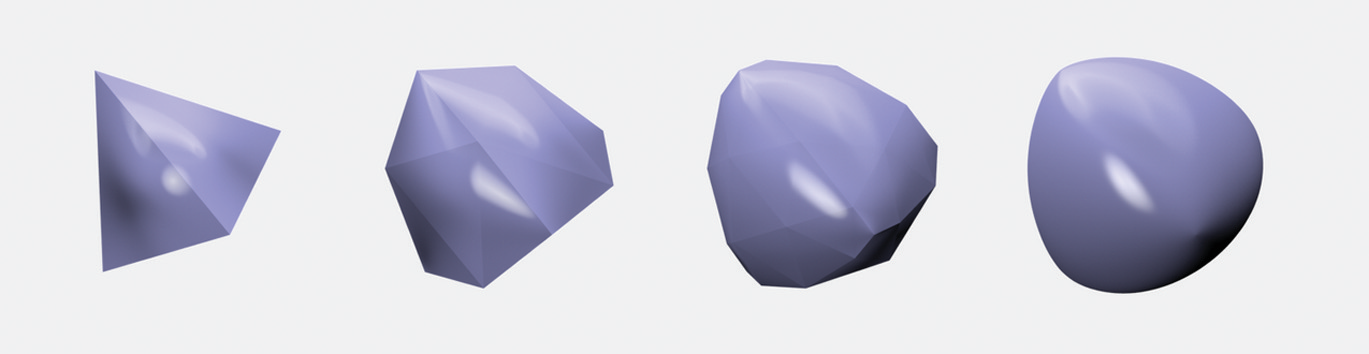
\includegraphics[width=\linewidth]{chap03/tetsubdiv.png}
    \caption{四面体的细分。从左到右使用了零步、一步、两步和六步细分
        (在零级时,顶点只是移动到极限曲面上)。
        随着细分得越来越多,网格逼近极限曲面,即原始网格描述的光滑曲面。
        随着执行更多级别的细分,注意高光如何变得更加准确、轮廓边缘如何变得更加平滑。}
    \label{fig:3.24}
\end{figure}

\reffig{3.25}展示了对Killeroo\sidenote{译者注:猜测此名字与一澳大利亚漫画中的袋鼠角色名有关。}模型应用细分的效果;
上面是原始控制网格,下面是控制网格表示的细分曲面。
\begin{figure}[htbp]
    \centering
    \subfloat[控制网格]{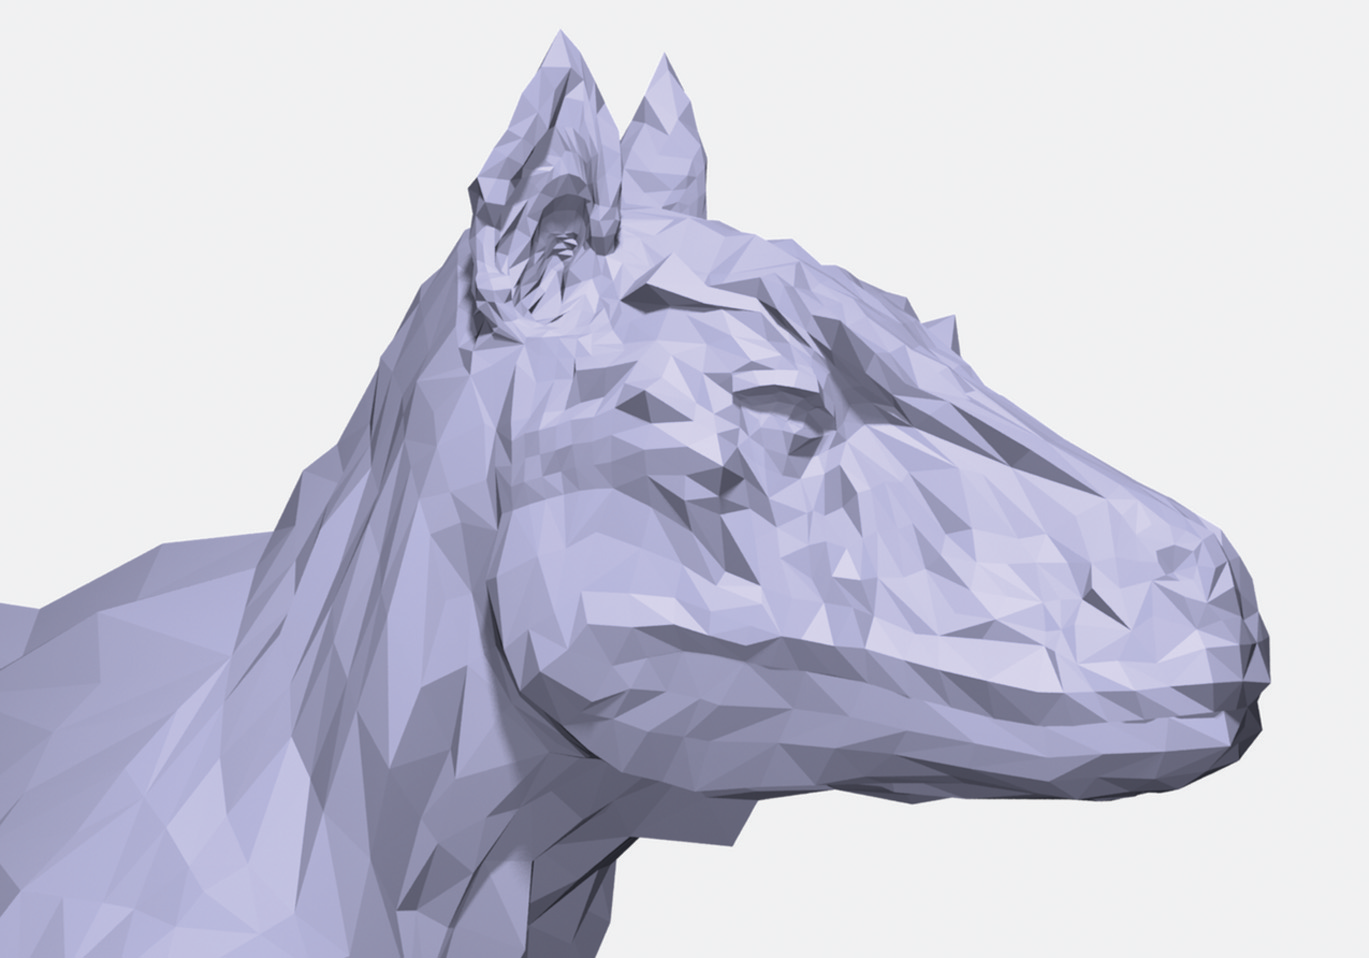
\includegraphics[width=\linewidth]{chap03/killeroo-control.png}\label{fig:3.25.1}}\\
    \subfloat[细分网格]{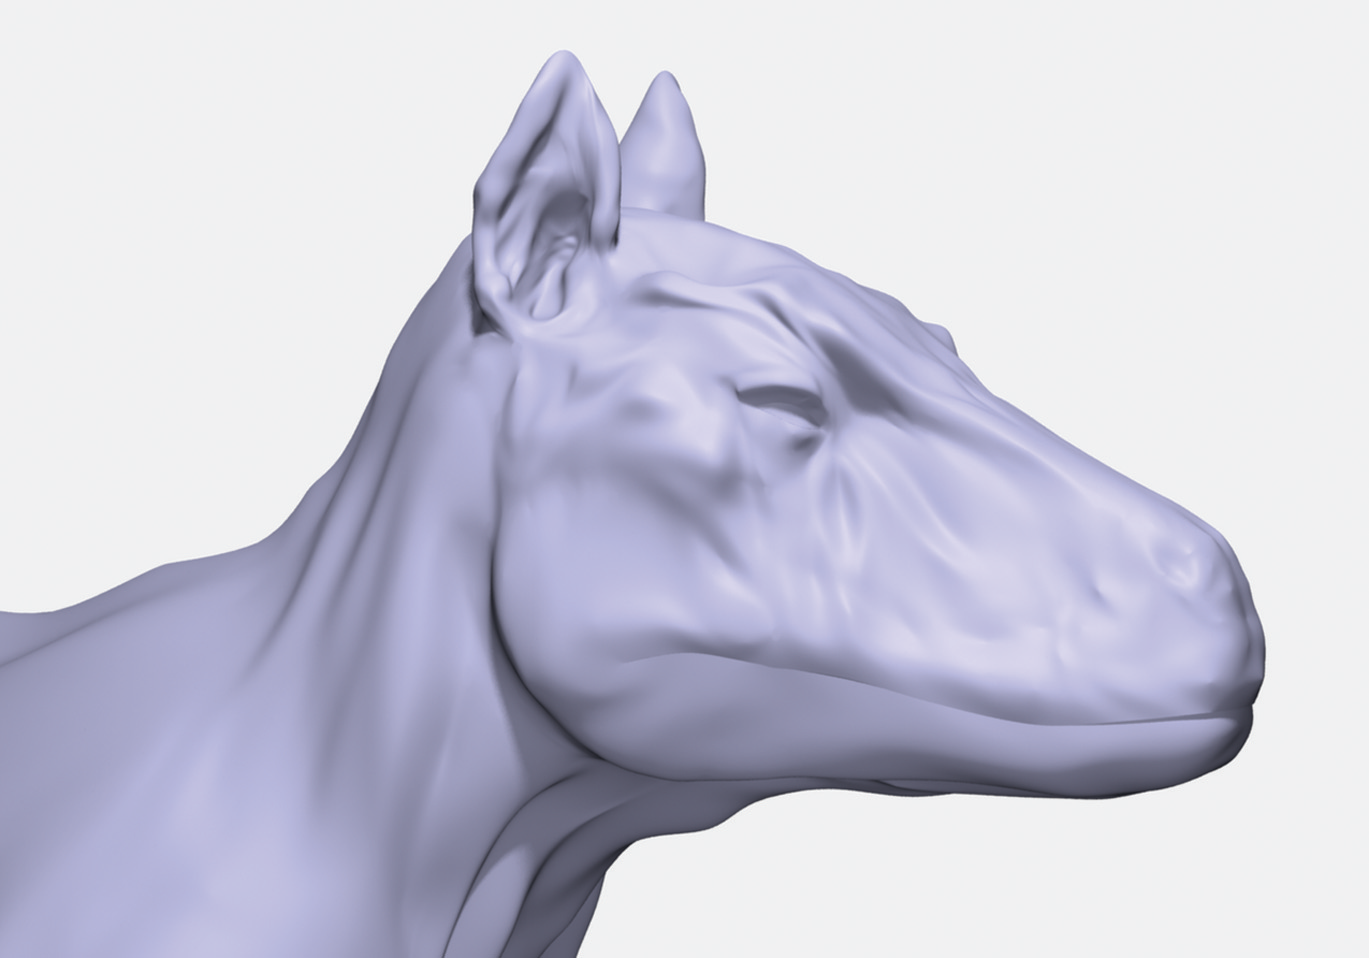
\includegraphics[width=\linewidth]{chap03/killeroo-subdivided.png}\label{fig:3.25.2}}
    \caption{对Killeroo模型应用细分。(1)控制网格描述了(2)结果细分曲面。
        细分非常适合建模这样的形状,因为它能通过细化控制网格轻松添加局部细节,
        对最终曲面没有拓扑结构限制。(模型由headus/Rezard提供。)}
    \label{fig:3.25}
\end{figure}


因为在曲面的多边形和基于样条的表示方面有一些重要优势,
细分曲面近年来得到广泛运用,尽管它在20世纪70年代就被发明了。
细分的优势包括:
\begin{itemize}
    \item 细分曲面是平滑的,而多边形网格与之相反,无论建模得多细致,靠近观察会有小面。
    \item 建模系统中现有的多数基本结构可以重定向到细分。
          建模多边形网格的经典技术工具箱可以应用到建模细分控制网格上。
    \item 细分曲面非常适合描述有复杂拓扑结构的物体,
          因为它们以任意(\keyindex{流形}{manifold}{})拓扑结构的控制网格为起点。
          参数化曲面模型一般不能很好地处理复杂拓扑结构。
\end{itemize}
\subsection{细分}\label{sub:细分}
